\documentclass[12pt]{article}

\usepackage{graphicx}
\graphicspath{{../Fichier_Image}}

\title{Hypothèse 6. Carrefour et Croisements}
\author{Thibault Clodion}

\begin{document}

\maketitle % Permet d'afficher le titre, l'author etc

\underline{Hypothèse :} Les croisements (carrefour) augmente le temps de sortie si il génère des flux opposés
\newline\newline
\underline{Expérience :}Enlever le carrefour exp 4. + Enlever le carrefour exp 7. (expliciter dans 3.(c)) + Enlever les deux portes en face dans l'exp 1.
\newline
Parler aussi du faite qu'il faut donc que les portes soient eloignés les unes des autres pour ne pas générer de carrefour inutile.
\newline

6. 4 avec Carrefour
\newline\newline
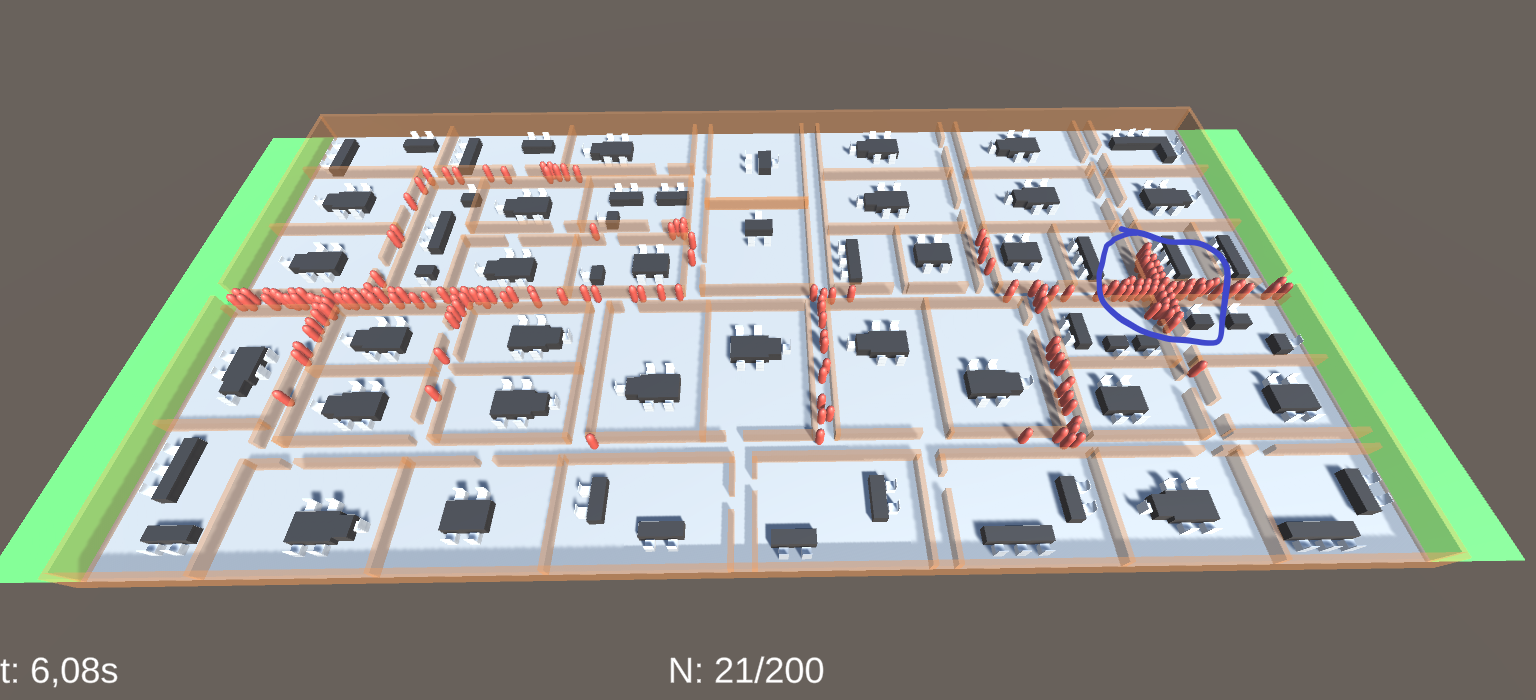
\includegraphics[scale=0.3]{6. 4 avec Carrefour.png}
\newline\newline
Temps moyen de dernière sortie : 24.79s
\newline
$\hspace*{0.2cm}$- Il y a un très grand flux au niveau du carrefour. (ce qui est négatif)
\newline
$\hspace*{0.2cm}$- Les deux flux s'opposent et tentent de rentrer dans le couloir ce qui entraîne une perte de fluidité dans ce dernier.
\newline\newline

6. 4 sans Carrefour
\newline\newline
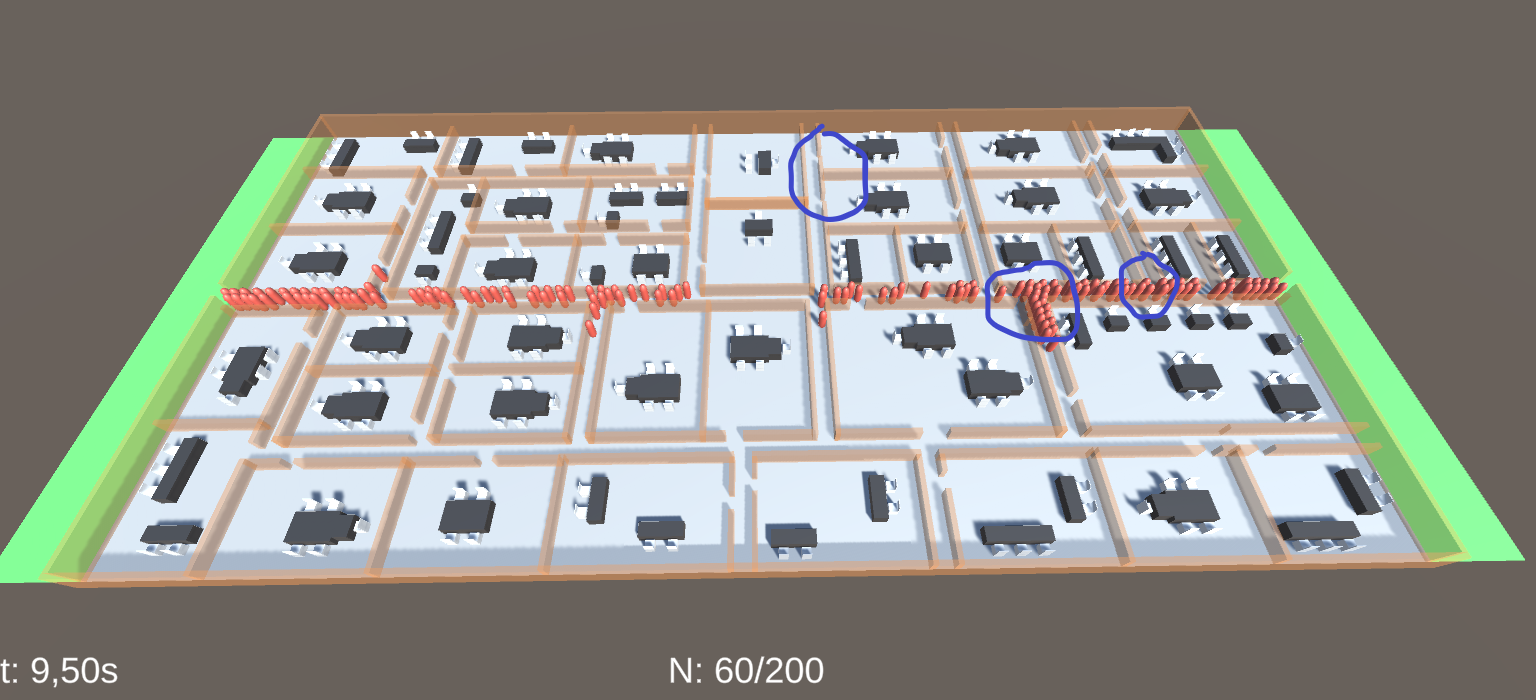
\includegraphics[scale=0.3]{6. 4 sans Carrefour .png}
\newline\newline
Temps moyen de dernière sortie : 23.23s
\newline
$\hspace*{0.2cm}$- Les 3 changements apportés permettent d'enlever la présence de croisements et flux opposés.
\newline
$\hspace*{0.2cm}$- On observe une plus grande fluidité dans les couloirs malgrés quelque ralentissement avant de rentrer dans le couloir principal.
\newline\newline

6. 7 avec Carrefour
\newline\newline
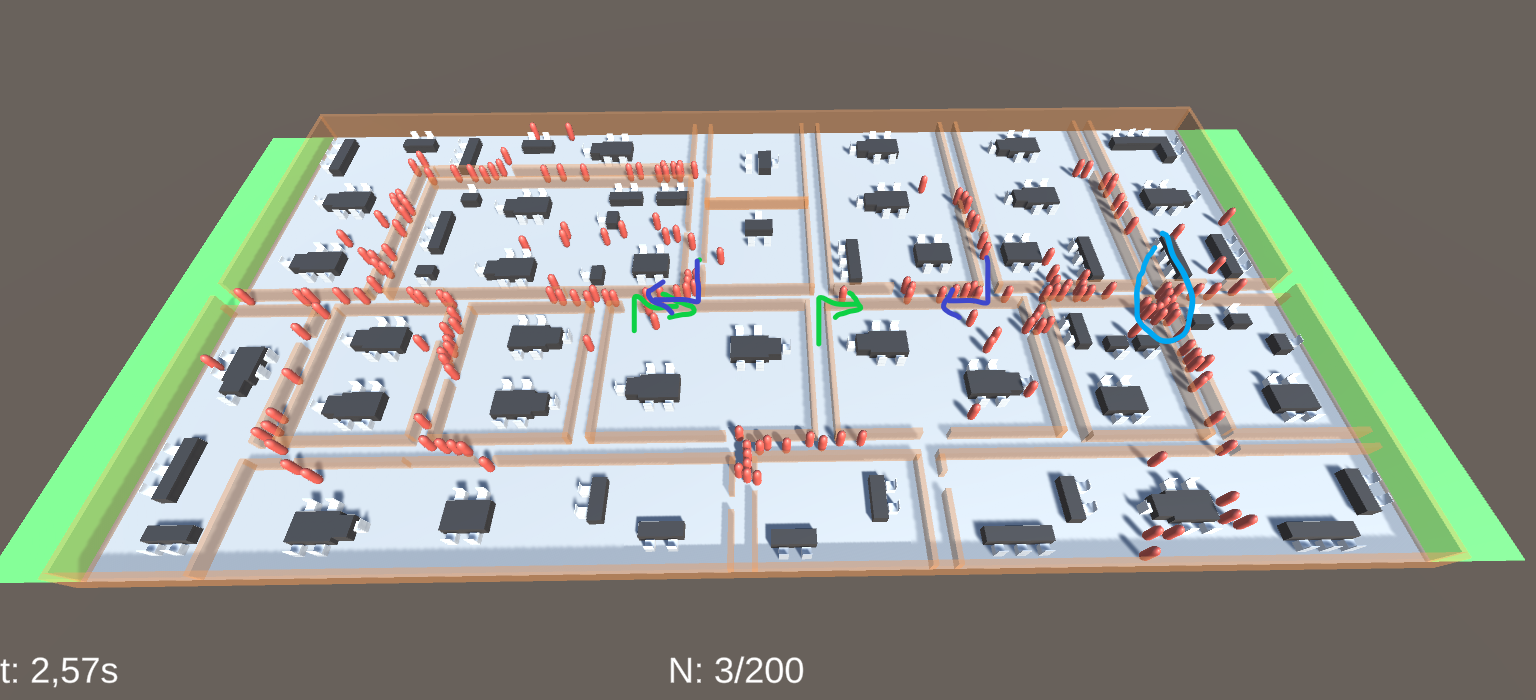
\includegraphics[scale=0.3]{6. 7 avec Carrefour.png}
\newline\newline
Temps moyen de dernière sortie : 23.72s
\newline
$\hspace*{0.2cm}$- On retrouve le carrefour introduit précedemment, mais également certains flux qui s'opposent.
\newline
$\hspace*{0.2cm}$- Le carrefour et les flux opposés génèrent beaucoup de ralentissements
\newline\newline

6. 7 sans Carrefour
\newline\newline
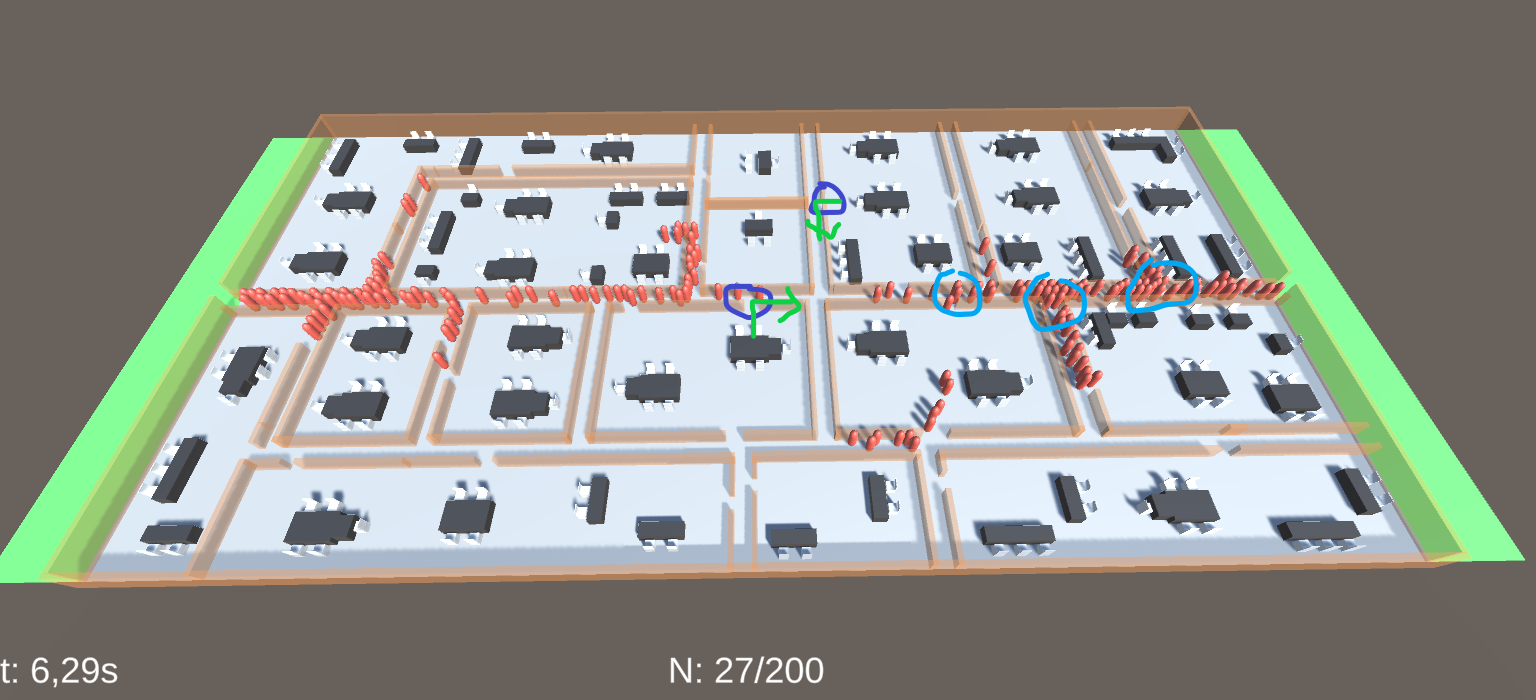
\includegraphics[scale=0.3]{6. 7 sans Carrefour.png}
\newline\newline
Temps moyen de dernière sortie : 22.93s
\newline
$\hspace*{0.2cm}$- Le fait d'avoir enlevé les carrefours, fluidifie l'arrivé dans le couloir principal même si l'importance du flux créer quelque ralentissement.
\newline
$\hspace*{0.2cm}$- Avoir enlevé le problème des flux opposés est grandement profitable (c'est en faite le pire lorsque deux piétons se croisent avec l'un voulant aller à gauche et l'autre à droite).

6. 1 avec Carrefour
\newline\newline
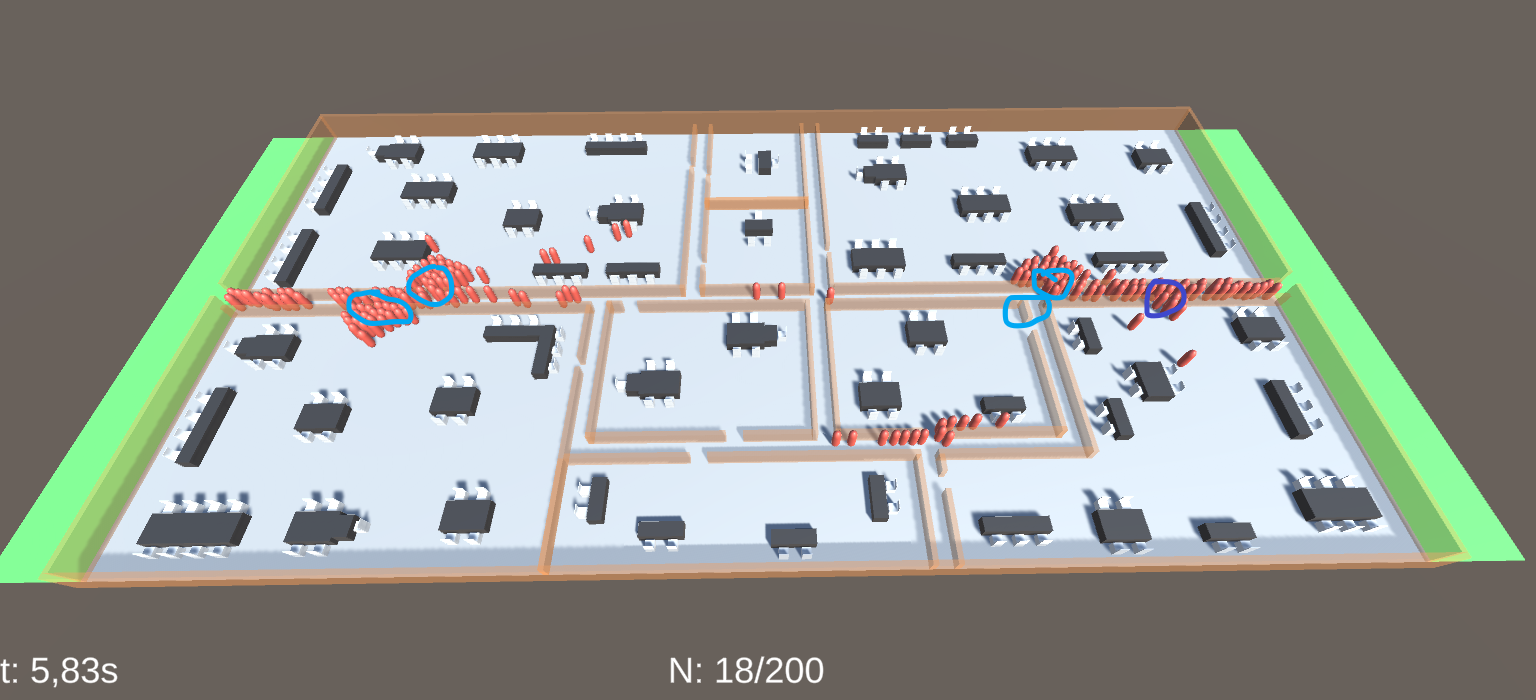
\includegraphics[scale=0.3]{6. 1 avec Carrefour.png}
\newline\newline
Temps moyen de dernière sortie : 24.51s
\newline
$\hspace*{0.2cm}$- Le but est ici de montrer qu'en éloignant les portes on divise les flux et améliore le temps de sorties.
\newline
$\hspace*{0.2cm}$- On pourra ainsi expliciter le fait qu'il faut éloigner au plus possible les portes des grand bureaux car sinon on a deux grand flux proches.
\newline
$\hspace*{0.2cm}$- En effet on a un grand ralentissement au niveau des zones bleus et particulièrement à gauche.
\newline\newline

6. 1 sans Carrefour
\newline\newline
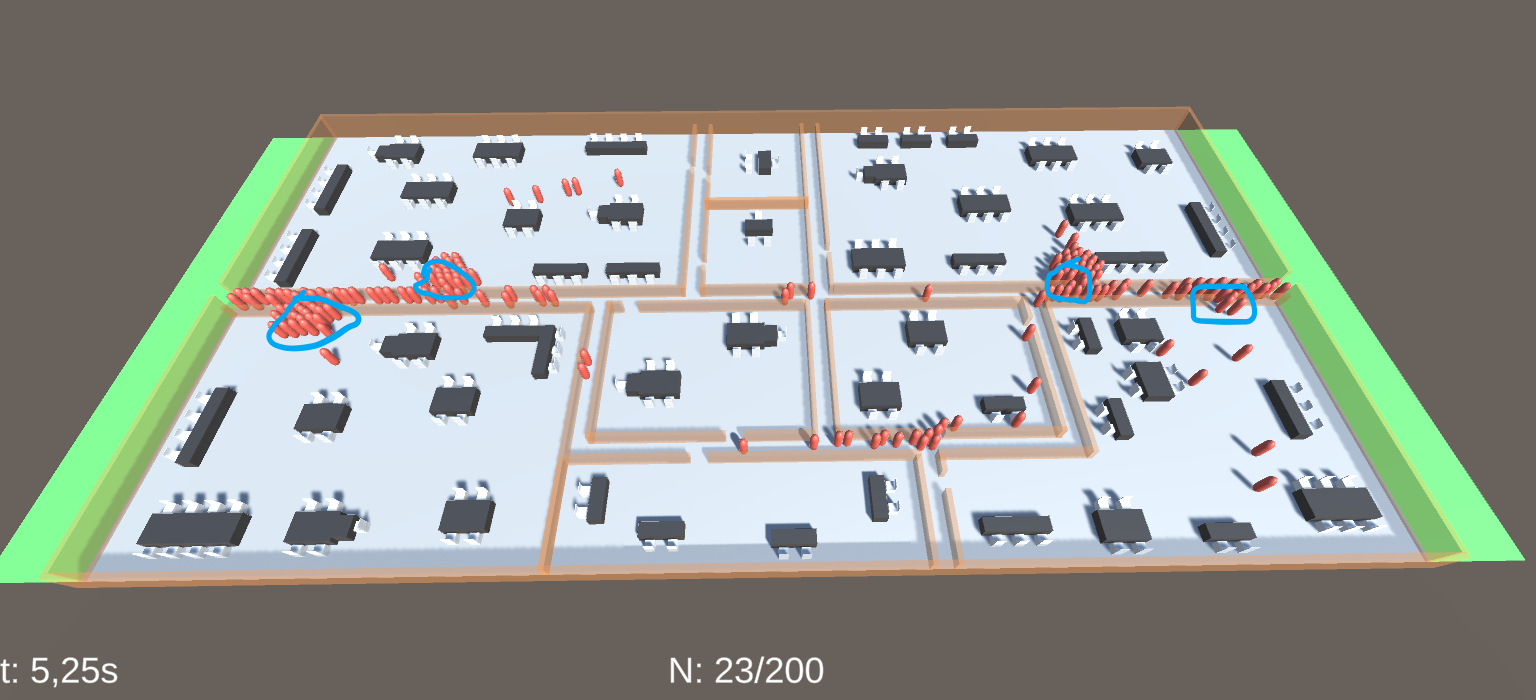
\includegraphics[scale=0.3]{6. 1 sans Carrefour.png}
\newline\newline
Temps moyen de dernière sortie : 23.18s
\newline
$\hspace*{0.2cm}$- On a donc éloigné les portes de sorties des bureaux
\newline
$\hspace*{0.2cm}$- On observe une plus grande fluidité au niveau du couloir principal et plus de flux opposés (en espérant que cela réduise le temps)
\newline\newline

\section{Résultats}
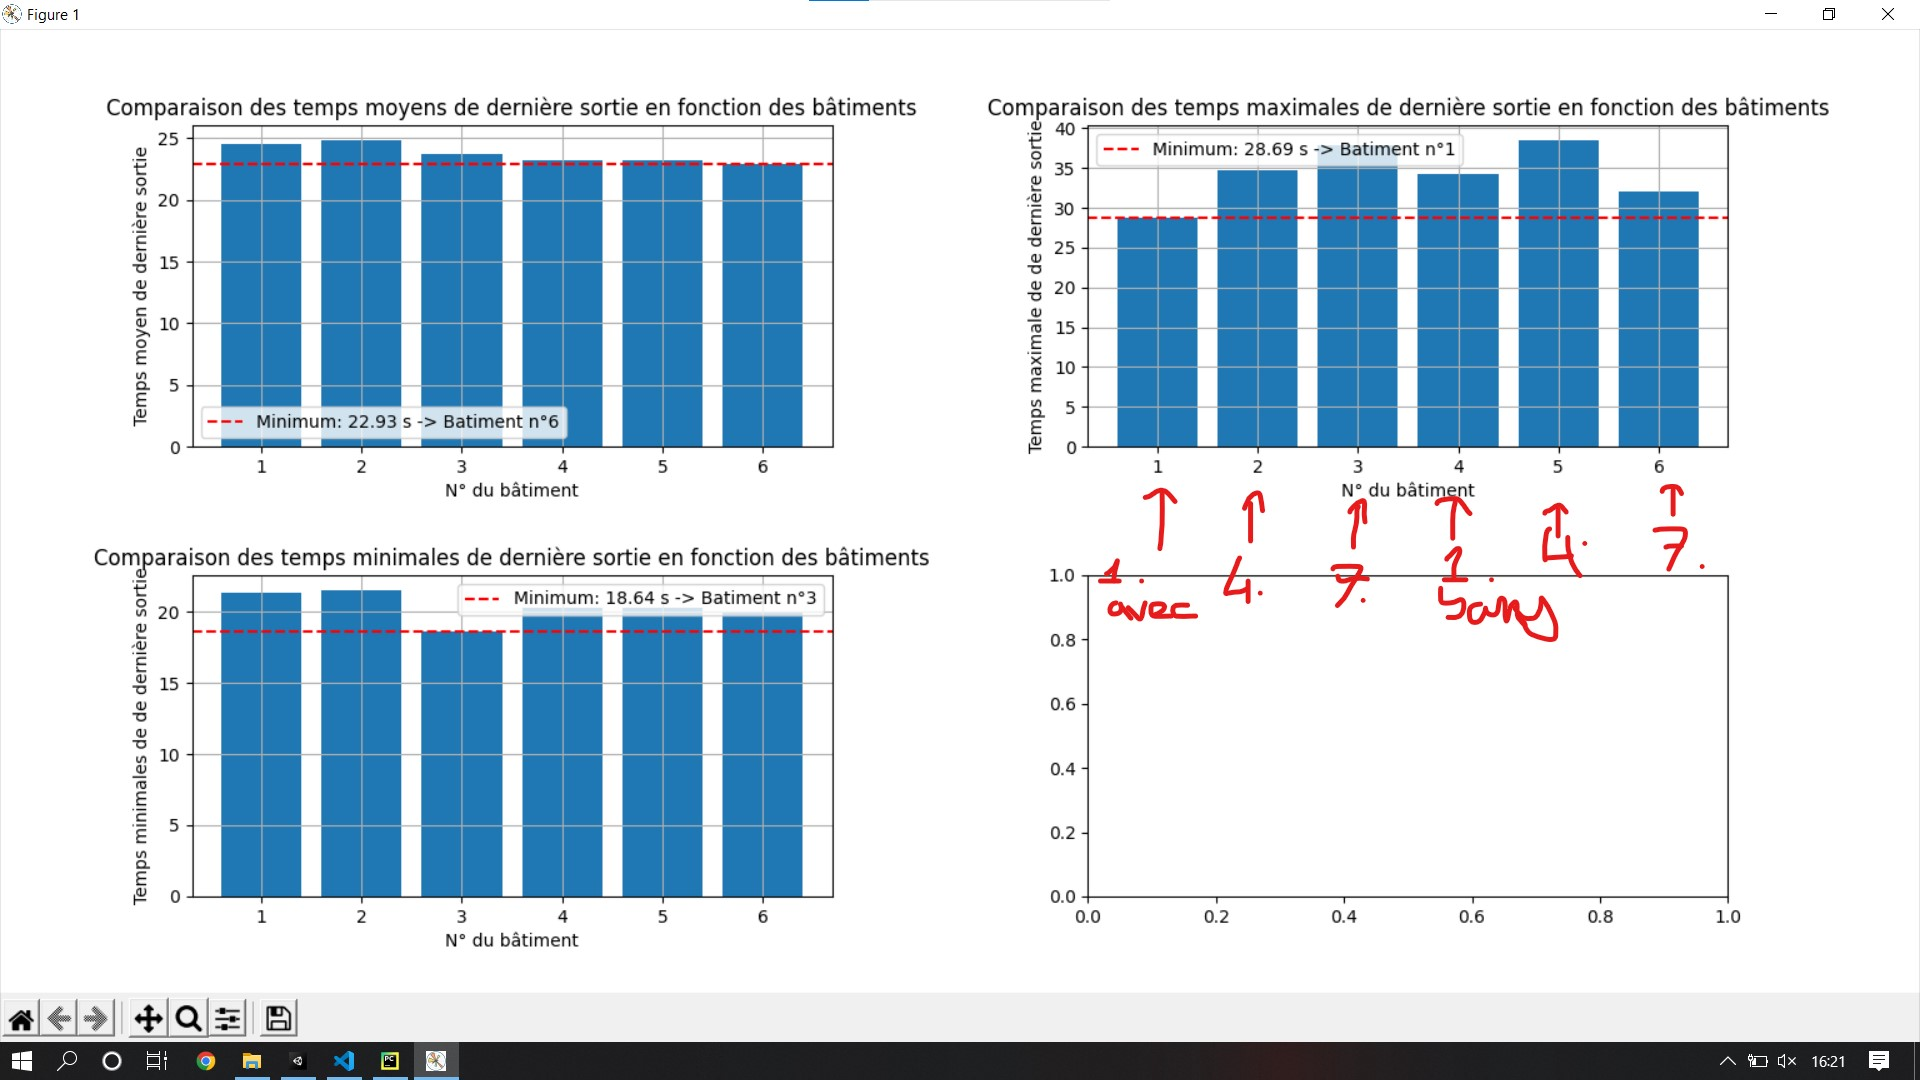
\includegraphics[scale=0.45]{6 - Resultat.jpg}
\newline\newline
On observe pour les 3 expériences que lorsque l'on enlève les croisements, on diminue le temps de sortie d'environ 1sec, c'est donc une hypothèse cruciale et validé !!


\end{document}